\documentclass[11pt]{article}
 
\usepackage[margin=1in]{geometry} 
\usepackage{amsmath,amsthm,amssymb}
\usepackage[framed,numbered,autolinebreaks,useliterate]{mcode}
\usepackage{graphicx}

\newcommand{\N}{\mathbb{N}}
\newcommand{\Z}{\mathbb{Z}}
 
\newenvironment{theorem}[2][Theorem]{\begin{trivlist}
\item[\hskip \labelsep {\bfseries #1}\hskip \labelsep {\bfseries #2.}]}{\end{trivlist}}
\newenvironment{lemma}[2][Lemma]{\begin{trivlist}
\item[\hskip \labelsep {\bfseries #1}\hskip \labelsep {\bfseries #2.}]}{\end{trivlist}}
\newenvironment{exercise}[2][Exercise]{\begin{trivlist}
\item[\hskip \labelsep {\bfseries #1}\hskip \labelsep {\bfseries #2.}]}{\end{trivlist}}
\newenvironment{problem}[2][Problem]{\begin{trivlist}
\item[\hskip \labelsep {\bfseries #1}\hskip \labelsep {\bfseries #2.}]}{\end{trivlist}}
\newenvironment{question}[2][Question]{\begin{trivlist}
\item[\hskip \labelsep {\bfseries #1}\hskip \labelsep {\bfseries #2.}]}{\end{trivlist}}
\newenvironment{corollary}[2][Corollary]{\begin{trivlist}
\item[\hskip \labelsep {\bfseries #1}\hskip \labelsep {\bfseries #2.}]}{\end{trivlist}}
 
\begin{document}
 
% --------------------------------------------------------------
%                         Start here
% --------------------------------------------------------------
 
\title{ECE 549 Computer Vision: Homework 1}%replace X with the appropriate number
\author{Xianming Liu\\ %replace with your name
NetID: xliu102} %if necessary, replace with your course title
 
\maketitle
 
\section{Lighting}

Answers:

\textbf{A}.
\begin{itemize}
\item[1.] Light from Right Above
\item[2.] It is because of Reflection, and more specifically, nearly specular reflection.
\item[3.] The cause of hard streaks is albedo. 
\item[4.] It is not possible that the glasses cast a shadow on it. If it is completely specular reflection, no light will be reflected to camera sensors and the whole table will be black.
\end{itemize}

\textbf{B}.
\begin{itemize}
\item[a.] If the surface has a specular component, the observed insensitive will change. Since for diffuse reflection, intensity is not dependent on view angle. But for specular reflection, the intensity will change. When the camera's view angle is on the specular reflection direction of a plane, the intensity of the point on the plane will be enhanced because more light is reflected (specularly) to camera sensor.
\item[b.] If the surface is Lambertian, then $I(x)= \rho(x)(\mathbf{S} \cdot N(x))$, in this case, 
\[
I_3 = I_2 \cdot \cos(\pi - \theta_{23}) = I_2 \sin(\theta_{23})
\], 
and 
\[
I_1 = I_2 \cdot \cos(\pi - \theta_{12}) = I_2 \sin(\theta_{12})
\].
So, to compute the angles, should use $\sin(\theta_{12}) = \frac{I_1}{I_2}$, and $\sin(\theta_{12}) = \frac{I_3}{I_2}$.
Given intensity vector $(0.5,0.9,0.8)$, we know $\sin(\theta_{12}) = 0.5/0.9$, $\theta_{12} = \arcsin(0.5/0.9)=0.59$, and $\sin(\theta_{23}) = 0.8/0.9$, $\theta_{23} = \arcsin(0.8/0.9)=1.09$ (in rad).
\end{itemize}

\section{Image Pyramids}
The Matlab codes are shown in the following:

% Or using
\lstinputlisting{"./code/gaussian_pyramids.m"}

and the main script is:
\lstinputlisting{"./code/pyramid_main.m"}

Figure~\ref{fig:pyramid} and Figure~\ref{fig:fft} show the results generated from the above code.

\begin{figure}[h]
\centering
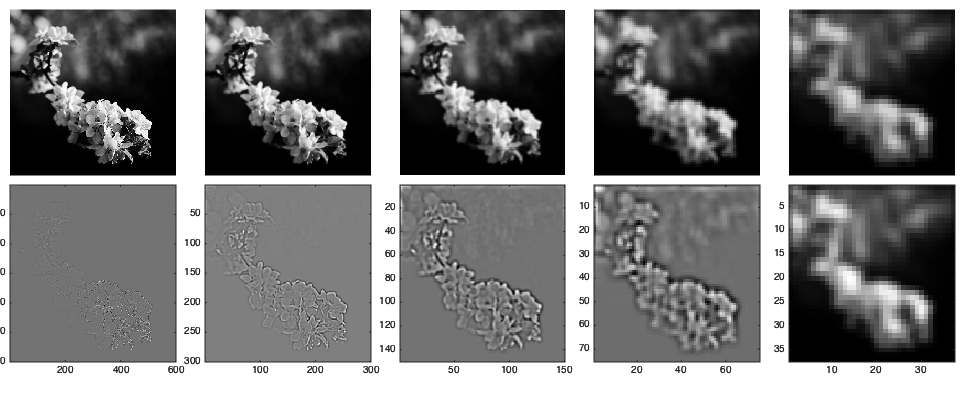
\includegraphics[width=0.95\linewidth]{./img/pyramid.png}
\caption{Gaussian and Laplacian Pyramid}
\label{fig:pyramid}
\end{figure}

\begin{figure}[h]
\centering
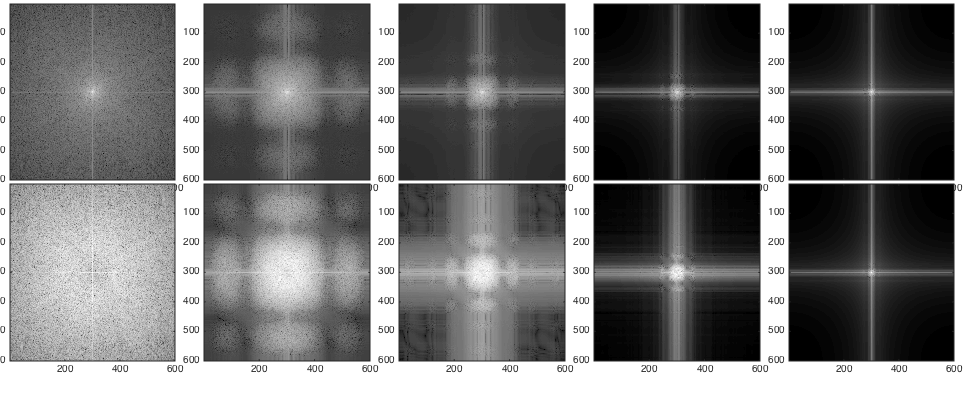
\includegraphics[width=0.95\linewidth]{./img/fft_mag_pyramid.png}
\caption{FFT Magnitude of Gaussian and Laplacian Pyramid}
\label{fig:fft}
\end{figure}

\textbf{Conclusion}: The \emph{Gaussian Pyramid} removes high frequencies signals in the image gradually, while \emph{Laplacian Pyramid} tries to preserve the lost high-frequency signals in the Gaussian Pyramid, in each level.

\section{Edge Detection}
\begin{description}
\item[a)] \emph{Gradient Edge}: In this implementation, the Gaussian Kernel size is $1$, and Gaussian filter size is $9*9$.

\item[b)] \emph{OrientedGradientMap}: In my implementation, I adopt Steerable Filters, on \emph{six} orientations. The filter bank is shown in Figure~\ref{fig:filter_bank}. For each filter, the kernel size is $\sqrt{2}$.

\begin{figure}[h]
\centering
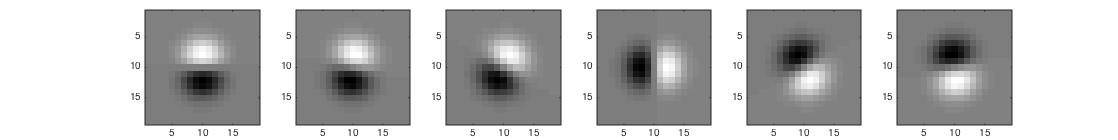
\includegraphics[width=0.95\linewidth]{./img/steerablefilters.png}
\caption{Steerable Filter bank used in orient boundary detection.}
\label{fig:filter_bank}
\end{figure}

\textbf{Qualitative Results}: As shown in Figure~\ref{fig:examples}, the boundary detected by orient filters are less noisy. Especially in the second example, the flower is detected by orient filters, but the edge response of gradient based method is not significant. 

\begin{figure}[h]
\centering
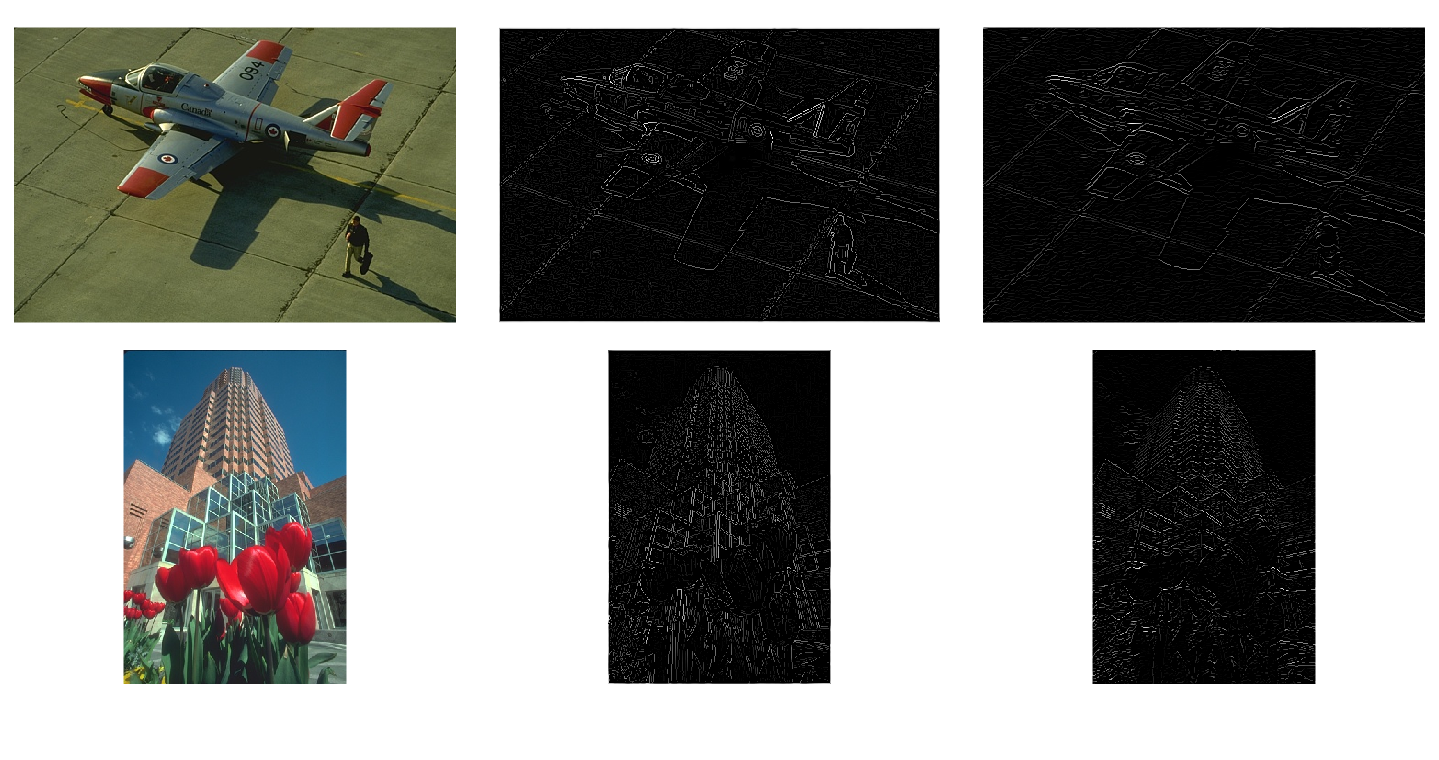
\includegraphics[width=\linewidth]{./img/examples.png}
\caption{Two examples of gradient based and orient filter based boundary detection. The second column is gradient based algorithm, and the third one is orient filter based results.}
\label{fig:examples}
\end{figure}

\textbf{Quantitative results}: PR curves for gradient-based and orient filter based methods are shown in Figure~\ref{fig:pr_gradient} and Figure~\ref{fig:pr_orient}. Quantitatively, orient filter based method performs better than gradient based method. More detail, Method gradient: overall F-score = $0.537$, average F-score = $0.564$; Method oriented: overall F-score = $0.536$, average F-score = $0.587$. 

\begin{figure}
\begin{minipage}{0.5\textwidth}
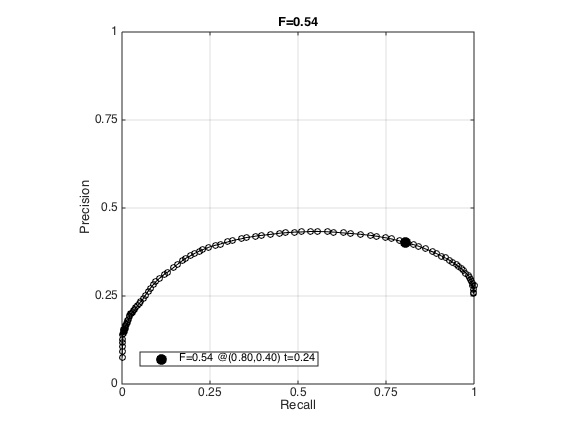
\includegraphics[width=\linewidth]{./img/pr_full_gradient.png}
\caption{PR curve of gradient based method}
\label{fig:pr_gradient}
\end{minipage}
\quad
\begin{minipage}{0.5\textwidth}
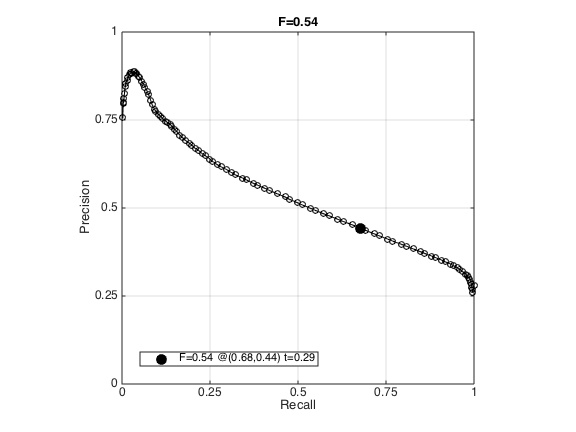
\includegraphics[width=\linewidth]{./img/pr_full_orient.png}
\caption{PR curve of orient filter based method}
\label{fig:pr_orient}
\end{minipage}
\end{figure}


\item[c)] \emph{Potential Improvement}: Edge responses may vary greatly on different scales. So, one possible improvement is to select the best scale for edge responses. Previous work \cite{ren2008multi} has already demonstrated the improvement of involving multiple scale filters in boundary detection. However, it is still computational heavy to extract features on so many scales. Inspired by Tony Lindeberg \cite{lindeberg1998feature} and my own work on scale selection for edges \cite{liu2012scale}, I implemented a simplified version of scale selection. The basic idea is to convolve the image with filters on multiple scales (5 in my implementation), and according to \cite{lindeberg1998feature}, a Gaussian normalizer should be used to obtain the normalized gradient response, by $L_{\sigma} = \sqrt{\sigma} \cdot L$, where $L$ is the oriented Laplacian of Gaussian responses. 

\item[d)]  As mentioned above, I implemented a scale-selective version of oriented filter based method. The F score improves slightly: Method multi scale oriented: overall F-score = 0.552, average F-score = 0.595. Figure~\ref{fig:pr_ms} shows the PR-Curve of the newly proposed method. In my complex implementation in \cite{liu2012scale}, I achieved average F-score = 0.66, with much less computation compared with \cite{ren2008multi}.

\begin{figure}[htb]
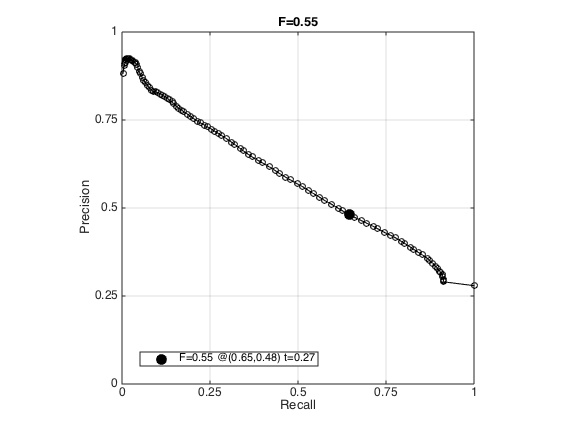
\includegraphics[width=0.5\linewidth]{./img/pr_full_ms.png}
\caption{PR curve of multi-scale orient filter based method}
\label{fig:pr_ms}
\end{figure}

\end{description}

\bibliographystyle{IEEEbib}
\bibliography{ref}
 
\end{document}